\documentclass[11pt,a4paper]{article}

\usepackage[T1]{fontenc}
\usepackage[utf8]{inputenc}
\usepackage{lmodern}
\usepackage[margin=2.4cm]{geometry}
\usepackage{microtype}
\usepackage{booktabs}
\usepackage{caption}
\usepackage{enumitem}
\usepackage{xcolor}
\usepackage{pgfplots}
\pgfplotsset{compat=1.17}
\usepackage[hidelinks]{hyperref}

\setlist{itemsep=2pt,topsep=4pt}
\captionsetup{font=small,labelfont=bf}
\newcommand{\code}[1]{\texttt{#1}}
\definecolor{plain}{HTML}{B4442F}
\definecolor{nottl}{HTML}{D49A2A}
\definecolor{hard}{HTML}{2F6DB4}

\title{\textbf{Leakage, Poisoning and Evasion:\\Auditing a Machine-Learning Intrusion Detector on UNSW-NB15}}
\author{Guerfi Ahmed Yacine\\
\small École Supérieure en Informatique de Sidi Bel Abbès (ESI-SBA), Algeria\\
\small \href{mailto:ay.guerfi@esi-sba.dz}{ay.guerfi@esi-sba.dz} \quad
\href{https://github.com/N4khlA/AI-_threat_hunting}{github.com/N4khlA/AI-\_threat\_hunting}}
\date{Technical report, November 2026}

\begin{document}
\maketitle

\begin{abstract}
\noindent
Machine-learning intrusion detectors are usually judged by one number on a
benchmark split, and treated as trusted components once deployed. This
report audits both assumptions on a Random Forest flow classifier trained on
UNSW-NB15. First, the evaluation: about 40\% of the dataset's rows are exact
duplicates, and a random re-split puts copies of the same flow in training
and test. Moving to the official split, with test flows restricted to those
never seen in training, lowers macro-F1 from 0.948 to 0.818 and raises the
false-positive rate at threshold 0.5 from 5.3\% to 26.5\%; the same leak
inflated a BiLSTM's AUC to 0.998. Second, the detector as a target. An
unauthenticated label field in the scoring API allowed training-data
poisoning: 2\% poisoned rows cut Backdoor recall from 1.00 to 0.67 while
overall accuracy rose, so an aggregate-metric retrain guard accepted the
model. On evasion, an attacker who only chooses their initial IP TTL evades
the plainly trained model on 100\% of detected attacks, because TTL is a
testbed artifact that the model uses as a shortcut. Dropping the TTL
features and adding adversarial training reduces evasion to at most 3.3\%
across all budgets tested, at a cost of 0.005 macro-F1. Every number is
regenerated by a script in the repository.
\end{abstract}

\section{Introduction}

Benchmark results for ML-based network intrusion detection are often
near-perfect, yet these systems are rarely trusted in production. Sommer and
Paxson~\cite{sommer2010} and Arp et al.~\cite{arp2022} attribute much of this
gap to evaluation pitfalls such as data snooping, spurious correlations and
unrealistic base rates; Kapoor and Narayanan~\cite{kapoor2023} show the same
leakage problems across ML-based science. A second gap is that a deployed
detector is itself software with an attack surface: its training data, its
retraining loop and its inputs can all be manipulated~\cite{biggio2018}.

This project started as a conventional detector (v1) that reported
macro-F1 0.948 for a Random Forest and AUC 0.998 for a BiLSTM on
UNSW-NB15~\cite{moustafa2015}. This report documents a systematic audit of
that system and the fixes that followed. Its contributions are:

\begin{enumerate}
  \item An evaluation audit across five split protocols that isolates how
        much of the headline score came from duplicates and split choice
        (\S\ref{sec:leakage}), and what the remaining performance means at
        realistic base rates (\S\ref{sec:baserate}).
  \item A label-poisoning proof of concept against the system's own
        retraining loop, and a per-family guard that blocks it
        (\S\ref{sec:poisoning}).
  \item A black-box evasion benchmark with physically plausible,
        attacker-side perturbations, which exposes TTL as a shortcut
        feature (\S\ref{sec:evasion}).
  \item A hardened model (no TTL features, adversarial training) that is
        now the one served, with its accuracy cost measured
        (\S\ref{sec:hardening}).
\end{enumerate}

\section{System and data}

\paragraph{Dataset.} UNSW-NB15~\cite{moustafa2015} contains network flows
from a 2015 testbed, described by 49 Argus/Bro features (45 numeric,
4 categorical), with nine attack families. We use the cleaned CSV release
(257,673 records, 63.9\% attacks), which provides an official training file
and an official testing file captured in different periods, but no IP
addresses or timestamps.

\paragraph{Model and pipeline.} The main detector is a Random Forest
(100 trees, unlimited depth, \code{min\_samples\_split}=5) trained on
imputed, encoded and scaled features with SMOTE oversampling on the training
set only. A separate Random Forest classifies the attack family for
alerting, and a bidirectional LSTM scores windows of 10 consecutive flows.
The model is served by a FastAPI service that emits alerts with a severity,
a MITRE ATT\&CK mapping and the exact per-feature decision-path
contributions of the forest.

\paragraph{Operating point.} Unless stated otherwise, thresholds are chosen
on a stratified 15\% validation split of the official training file so that
validation FPR $\le$ 1\%, then applied unchanged to the test set.

\section{Evaluation leakage}
\label{sec:leakage}

The v1 pipeline merged both files and re-split them at random 70/15/15.
Because 40\% of rows are exact duplicates, many test flows had identical
twins in training. We evaluated the same model and hyperparameters under
five protocols (Table~\ref{tab:protocols}); 95\% confidence intervals are
percentile bootstraps over test rows.

\begin{table}[h]
\centering
\small
\caption{One Random Forest, five evaluation protocols. \emph{Novel} restricts
the test set to flows with no exact copy in training (74,072 duplicate training
rows, 28,380 duplicate test rows and 1,304 test rows seen in training removed).
The last row is the served model.}
\label{tab:protocols}
\begin{tabular}{@{}lrlrr@{}}
\toprule
Protocol & Test rows & Macro-F1 [95\% CI] & ROC-AUC & FPR@0.5 \\
\midrule
Random re-split (v1)              & 38,651 & 0.948 [0.945, 0.950] & 0.992 & 5.3\% \\
Random re-split, deduplicated     & 23,115 & 0.917 [0.914, 0.922] & 0.981 & 7.6\% \\
Official train $\to$ test         & 82,332 & 0.862 [0.860, 0.865] & 0.981 & 27.5\% \\
\textbf{Official, novel test}     & 52,648 & \textbf{0.818} [0.815, 0.822] & 0.963 & 26.5\% \\
Official, novel, no TTL features  & 52,648 & 0.816 [0.813, 0.819] & 0.961 & 26.8\% \\
Official, novel, hardened (served)& 52,648 & 0.813 [0.810, 0.817] & 0.960 & 27.5\% \\
\bottomrule
\end{tabular}
\end{table}

Three observations follow.
\begin{itemize}
  \item \textbf{The split, not the model, explains about 13 F1 points.}
        Deduplication alone costs 3 points; testing on the other capture
        period costs most of the rest, and the false-positive rate at 0.5
        rises five-fold because benign traffic differs between captures.
  \item \textbf{Feature importance is not feature necessity.} The two most
        important features are \code{sttl} and \code{ct\_state\_ttl}, both
        derived from the IP time-to-live, a known artifact of the UNSW-NB15
        testbed. Removing all three TTL features costs only 0.002 F1, since
        other features carry the same separation. Section~\ref{sec:evasion}
        shows that keeping them is nonetheless costly.
  \item \textbf{Thresholds do not transfer.} A threshold chosen for 1\% FPR
        on validation yields 4--5\% FPR on test.
\end{itemize}

The same leak affected the sequence model: with a stride of 5 and windows of
10, the v1 random window split placed 54,041 flows in both training and test
windows. Building windows per file removes the overlap and lowers the LSTM's
AUC from 0.998 to 0.989 and its F1 from 0.985 to 0.894. On the 10,544 flows
both models can score, the LSTM and the Random Forest are statistically tied
(accuracy 0.819 vs.\ 0.815, McNemar $p=0.27$). The v1 conclusion that the
LSTM was stronger was an artifact of the leak.

\section{What the remaining performance means in practice}
\label{sec:baserate}

At its operating threshold (0.880) the served model detects 76.5\% of
attacks at 4.3\% FPR. Following Axelsson~\cite{axelsson2000}, we translate
this into alert volumes for a network producing one million flows per day
(Table~\ref{tab:baserate}).

\begin{table}[h]
\centering
\small
\caption{Expected alerts per day for $10^6$ flows at the served operating point.}
\label{tab:baserate}
\begin{tabular}{@{}rrrr@{}}
\toprule
Attack prevalence & Alert precision & True alerts/day & False alerts/day \\
\midrule
1\%   & 15.2\% & 7,654 & 42,551 \\
0.1\% & 1.8\%  & 765   & 42,938 \\
\bottomrule
\end{tabular}
\end{table}

A model with 0.96 ROC-AUC still produces about 43,000 false alerts a day.
The system is therefore designed for human triage rather than automatic
blocking: alerts are ranked by severity and carry the features that drove
the verdict. Per-family recall at this threshold ranges from 0.96 (Generic)
to 0.23 (Fuzzers); Fuzzers traffic is designed to resemble benign flows and
remains the main weakness.

\section{Attack 1: label poisoning}
\label{sec:poisoning}

\paragraph{Vulnerability.} The v1 \code{/predict} endpoint accepted optional
\code{Label} and \code{attack\_cat} fields from any caller, stored them as
ground truth, and the retraining script trained on them (MITRE ATLAS~\cite{atlas}
AML.T0020). A candidate model replaced the incumbent if its accuracy or F1
improved.

\paragraph{Experiment.} The incumbent is a Random Forest trained on 60\% of
the training set (accuracy 0.816, Backdoor recall 1.00). Each candidate is
trained on the full training set, which also contains genuine new data, plus
$n$ attacker-submitted copies of Backdoor flows labelled benign.

\begin{table}[h]
\centering
\small
\caption{Targeted poisoning of the Backdoor family. Accuracy stays flat or
improves, so an aggregate-only guard accepts every poisoned model.}
\label{tab:poison}
\begin{tabular}{@{}rrrrcc@{}}
\toprule
Poison budget & Rows & Accuracy & Backdoor recall & v1 guard & v2 guard \\
\midrule
0\%    & 0     & 0.8208 & 1.000 & accept & accept \\
0.25\% & 221   & 0.8204 & 1.000 & accept & accept \\
0.5\%  & 441   & 0.8203 & 0.957 & accept & refuse \\
1\%    & 882   & 0.8196 & 0.829 & accept & refuse \\
2\%    & 1,764 & 0.8210 & 0.671 & accept & refuse \\
5\%    & 4,411 & 0.8181 & 0.614 & accept & refuse \\
\bottomrule
\end{tabular}
\end{table}

\paragraph{Result.} Table~\ref{tab:poison}: with 2\% poisoned rows, one in
three Backdoor flows goes undetected, while accuracy is higher than with no
poison at all. Because the candidate also benefits from genuine new data, the
v1 guard accepted every poisoned model.

\paragraph{Fixes.} (i)~The scoring schema rejects unknown fields, so a
\code{Label} on \code{/predict} returns HTTP~422. (ii)~Labels are accepted
only through a separate \code{/feedback} endpoint that requires an analyst
API key, references a logged prediction, and records who labelled it.
(iii)~Retraining uses only analyst labels; pseudo-labelling is opt-in.
(iv)~The v2 guard refuses any candidate whose recall on any attack family
drops by more than 0.02 relative to the incumbent, which catches the attack
from the 0.5\% budget onwards.

\section{Attack 2: evasion}
\label{sec:evasion}

\paragraph{Threat model.} A black-box attacker (ATLAS AML.T0015 / AML.T0043)
observes only whether a flow is flagged and controls only their own side of
the connection. Every perturbation adds cost without removing the attack:
padding payloads (\code{sbytes}), adding packets (\code{Spkts}, with header
bytes), slowing the flow (\code{dur} and inter-packet gaps), and choosing
the initial TTL, set to a value typical of benign traffic. Derived features
(\code{Sload}, \code{Dload}, \code{smeansz}, \code{Sintpkt}) are recomputed
so that records stay self-consistent; destination-side fields are untouched.
Each continuous knob is drawn from $[0,\varepsilon]$ as a relative increase,
with 40 random-search queries per flow. We attack 1,500 correctly detected
test attacks per model; success means the score falls below the model's
operating threshold.

\paragraph{Models.} \emph{Plain}: the v1 recipe on all features.
\emph{No-TTL}: the same without \code{sttl}, \code{dttl} and
\code{ct\_state\_ttl}. \emph{Hardened}: no TTL plus adversarial training
(\S\ref{sec:hardening}). The three have nearly identical clean performance
(TPR 0.787 / 0.779 / 0.778 at FPR 0.050 / 0.048 / 0.050).

\begin{figure}[h]
\centering
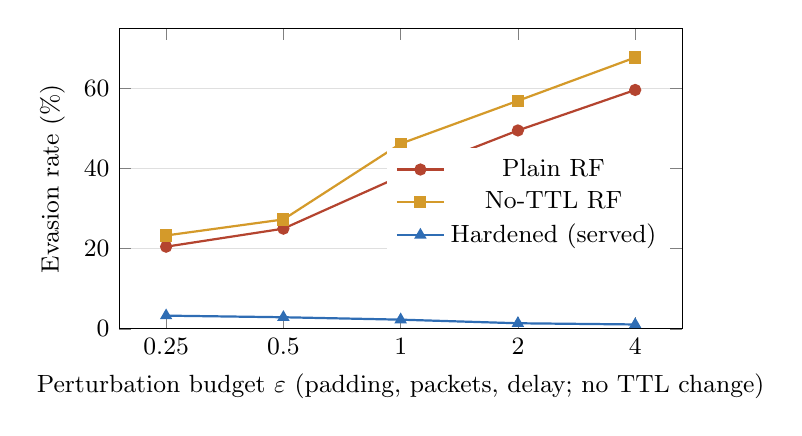
\begin{tikzpicture}
\begin{axis}[
  width=0.72\linewidth, height=5.4cm,
  xlabel={Perturbation budget $\varepsilon$ (padding, packets, delay; no TTL change)},
  ylabel={Evasion rate (\%)},
  xmode=log, log basis x=2,
  xtick={0.25,0.5,1,2,4}, xticklabels={0.25,0.5,1,2,4},
  ymin=0, ymax=75, ymajorgrids, grid style={gray!25},
  legend style={at={(0.98,0.42)}, anchor=east, font=\small, draw=none, fill=white},
  tick label style={font=\small}, label style={font=\small},
  every axis plot/.append style={thick, mark size=1.8pt},
]
\addplot[color=plain, mark=*] coordinates {(0.25,20.5) (0.5,25.0) (1,38.1) (2,49.5) (4,59.6)};
\addplot[color=nottl, mark=square*] coordinates {(0.25,23.3) (0.5,27.3) (1,46.2) (2,56.9) (4,67.7)};
\addplot[color=hard, mark=triangle*] coordinates {(0.25,3.3) (0.5,2.9) (1,2.3) (2,1.4) (4,1.1)};
\legend{Plain RF, No-TTL RF, Hardened (served)}
\end{axis}
\end{tikzpicture}
\caption{Share of detected attacks pushed below the operating threshold.
At $\varepsilon=0$ every model is at 0\%, which checks that the perturbation
code is an exact identity at zero budget.}
\label{fig:evasion}
\end{figure}

\paragraph{The TTL shortcut.} In UNSW-NB15, an observed \code{sttl} of 31
occurs only in benign rows. An attacker who sets their initial TTL so that
the sensor observes this value evades the plain model on \textbf{100\%} of
detected attacks, at every budget including $\varepsilon=0$. A single
attacker-controlled header field defeats the model. Section~\ref{sec:leakage}
showed that the TTL features are barely needed for accuracy; this experiment
shows they must be removed for robustness. Importance analysis alone would
not have revealed this.

\paragraph{Cheap perturbations.} Without TTL, padding and slowing still
evade 23--68\% of detections (Figure~\ref{fig:evasion}). The no-TTL model is
slightly \emph{easier} to evade with them than the plain one, presumably
because without the shortcut it leans more on the volume and timing features
that these perturbations change. Fuzzers (89\% evaded at
$\varepsilon=1$) and Analysis (74\%) are the easiest families to push over.

\section{Hardening}
\label{sec:hardening}

The served model combines two measures: it never sees the TTL features, and
its training set is augmented with perturbed copies of every training attack
(knobs drawn from $U(0,2)$, TTL drawn from benign-typical values), still
labelled as attacks~\cite{goodfellow2015}. The same module builds the
training set for initial training, retraining and evaluation, so the recipe
cannot drift between them.

\begin{table}[h]
\centering
\small
\caption{Evasion rate with TTL rewriting allowed, and clean cost of hardening.}
\label{tab:hardening}
\begin{tabular}{@{}lrrrrr@{}}
\toprule
Model & $\varepsilon=0$ & $\varepsilon=0.25$ & $\varepsilon=1$ & $\varepsilon=4$ & Macro-F1 (novel test) \\
\midrule
Plain RF          & 100\% & 100\% & 100\% & 100\% & 0.818 \\
No-TTL RF         & 0\%   & 23.1\% & 46.2\% & 66.7\% & 0.816 \\
\textbf{Hardened} & 0\%   & \textbf{3.2\%} & \textbf{1.9\%} & \textbf{1.3\%} & 0.813 \\
\bottomrule
\end{tabular}
\end{table}

Hardening reduces evasion to at most 3.3\% at every budget tested, with or
without TTL rewriting, for a cost of 0.005 macro-F1 (Table~\ref{tab:hardening}).
The worst remaining family is Fuzzers, at 10.5\% evasion for $\varepsilon=1$.
A regression test checks that changing \code{sttl} cannot change the served
model's score. This robustness holds only for the perturbation family the
model was trained on; Section~\ref{sec:limits} lists what is not covered.

\paragraph{Service hardening.} Beyond the model, the API was hardened against
the OWASP API Security Top~10: role-based API keys stored as SHA-256 digests
and compared in constant time, failing closed when none are configured; a
strict input schema that rejects unknown fields, NaN and out-of-range values;
per-key rate limiting and body-size caps; and SHA-256 pinning of every model
artifact and of the alert threshold, verified at startup on the exact bytes
that are then deserialised. The repository contains 108 automated tests,
with static analysis (\code{bandit}) and dependency auditing
(\code{pip-audit}) in continuous integration.

\section{Limitations}
\label{sec:limits}

\begin{itemize}
  \item \textbf{One synthetic dataset.} UNSW-NB15 is a 2015 testbed. No
        cross-dataset evaluation was run: the features of datasets such as
        CIC-IDS2017 barely overlap with UNSW-NB15's, so a transfer score
        would mostly measure feature mapping. The shift between the two
        official capture periods is the closest available proxy.
  \item \textbf{Weak sequence signal.} The cleaned release has no IP
        addresses or timestamps, so LSTM windows group flows by protocol and
        service in file order. Per-host sequences need the original files.
  \item \textbf{Limited adversary.} The evasion attacker uses random search
        over four knobs. An adaptive attacker who changes protocol, splits
        an attack across many flows, or optimises against the hardened model
        directly is out of scope.
  \item \textbf{No end-to-end capture.} The models need Argus features; the
        demo replays held-out flows rather than processing raw packet
        captures.
  \item \textbf{Operational gaps.} Thresholds must be recalibrated on the
        defended network, and an attacker able to rewrite both an artifact
        and its manifest defeats pinning unless the manifest is signed.
\end{itemize}

\section{Conclusion}

Most of this detector's original headline score came from the evaluation,
not the model: duplicates and a random split accounted for about 13 F1
points, and a sequence model's apparent advantage disappeared once training
and test windows stopped overlapping. Treating the detector as a target
exposed two further failures that standard metrics hide: a poisoning path
through the retraining loop that left accuracy unchanged, and a testbed
artifact that let one header field evade every detection. Both were fixed
at a measured cost of 0.005 macro-F1. The broader lesson is that leakage
audits, per-family metrics and adversarial testing belong in the evaluation
of security ML systems, not after it.

\paragraph{Reproducibility.} \code{scripts/reproduce.sh} regenerates every
table and figure in about 15 minutes on 8 CPU cores with fixed seeds. Each
report in \code{reports/} names the script that produced it
(\code{rigorous\_eval.py}, \code{poisoning.py}, \code{evasion.py},
\code{evaluate.py}).

\begin{thebibliography}{9}
\small
\bibitem{moustafa2015} N.~Moustafa and J.~Slay. UNSW-NB15: A comprehensive
data set for network intrusion detection systems. In \emph{Military
Communications and Information Systems Conference (MilCIS)}, 2015.

\bibitem{sommer2010} R.~Sommer and V.~Paxson. Outside the closed world: On
using machine learning for network intrusion detection. In \emph{IEEE
Symposium on Security and Privacy}, 2010.

\bibitem{arp2022} D.~Arp, E.~Quiring, F.~Pendlebury, A.~Warnecke, F.~Pierazzi,
C.~Wressnegger, L.~Cavallaro, and K.~Rieck. Dos and don'ts of machine learning
in computer security. In \emph{USENIX Security Symposium}, 2022.

\bibitem{kapoor2023} S.~Kapoor and A.~Narayanan. Leakage and the
reproducibility crisis in machine-learning-based science. \emph{Patterns},
4(9), 2023.

\bibitem{biggio2018} B.~Biggio and F.~Roli. Wild patterns: Ten years after the
rise of adversarial machine learning. \emph{Pattern Recognition}, 84, 2018.

\bibitem{goodfellow2015} I.~Goodfellow, J.~Shlens, and C.~Szegedy. Explaining
and harnessing adversarial examples. In \emph{International Conference on
Learning Representations (ICLR)}, 2015.

\bibitem{axelsson2000} S.~Axelsson. The base-rate fallacy and the difficulty
of intrusion detection. \emph{ACM Transactions on Information and System
Security}, 3(3), 2000.

\bibitem{atlas} MITRE. ATLAS: Adversarial Threat Landscape for
Artificial-Intelligence Systems. \url{https://atlas.mitre.org}.
\end{thebibliography}

\end{document}
